% Ubah judul dan label berikut sesuai dengan yang diinginkan.
% \section{Literature Review}
% \label{sec:relatedworks}

% Ubah paragraf-paragraf pada bagian ini sesuai dengan yang diinginkan.

% Update the title and label below as desired.

\section{Literature Review}
\label{sec:literaturereview}

\subsection{Previous Research}
\label{subsec:previousresearch}

Research conducted by Andi Aljabar and Suhartijo successfully translated Indonesian sign language using Convolutional Neural Network (CNN), Long Short-Term Memory (LSTM), and a combination of both architectures. Testing on 10 BISINDO vocabulary classes showed an average accuracy of 73\% for CNN, 81\% for LSTM, and 90\% for the CNN-LSTM combination \cite{aljabar2020}. Research by Husna Moetia Putri, Fadlisyah, and Wahyu Fuadi detected sign language in real-time using LSTM and MediaPipe Holistic. Evaluation on 10 BISINDO vocabularies achieved 92\% accuracy and 65\% accuracy for 30 vocabularies \cite{putri2022}. Siti Nur, Aghisna Nur Assyifa, and Habilah Nurjannah developed a BISINDO translator application using LSTM with an accuracy of 75\% on 500 data, increasing to 85\% on 1000 and 1500 data. This application has a feature to add vocabulary and save data to produce sign vocabulary output accordingly \cite{nur2023}.

\subsection{Indonesian Sign Language (BISINDO)}
\label{subsec:indonesiansignlanguage}

Deafness is the term for someone who has lost or is unable to receive auditory stimuli through their hearing senses \cite{mursita2015}. Based on birth, deafness can be divided into two: \emph{congenitally deaf} (from birth) and \emph{adventitiously deaf} (due to disease or traumatic events). Deafness is also classified based on hearing ability in decibels (dB), ranging from mild to total \cite{winarsih2007}. In Indonesia, at least 2.9 million people, or 1.25\% of the population, are deaf \cite{evitasari2015}. Deaf individuals use sign language for communication. Sign language is expressed through a combination of hand shapes, hand movement orientations, arm movements, and facial expressions \cite{mursita2015}. There are two sign languages that have developed in Indonesia: the Indonesian Sign Language System (SIBI) and Indonesian Sign Language (BISINDO). SIBI uses one hand, while BISINDO uses two. BISINDO is more commonly used because it is not bound to the structure of the Indonesian language and originates from the native language of the deaf, adapting to their understanding without emphasizing Indonesian language affixes.

\subsection{Mediapipe}
\label{subsec:mediapipe}

MediaPipe is a framework for building inference pipelines on sensory data such as audio and video. This framework enables the creation of pipelines consisting of modular components, such as inference models, media processing algorithms, and data transformations. MediaPipe abstracts and connects individual perception models into maintainable workflows, allowing components to be reused. MediaPipe's core concepts include a framework for sensory data inference, performance evaluation tools, and reusable processing components. MediaPipe is designed to support the development of machine learning and deep learning models, such as object detection and sign language movement detection \cite{lugaresi2019:}. MediaPipe Pose is a framework that can predict a total of 33 landmark locations, starting from the nose to the right leg. MediaPipe Hand is a framework that can predict 21 landmark locations covering the entire hand \cite{googleMediapipe}.

\subsection{\emph{Long Short-Term Memory} (LSTM)}
\label{subsec:lstm}

\begin{figure}[ht]
    \centering
    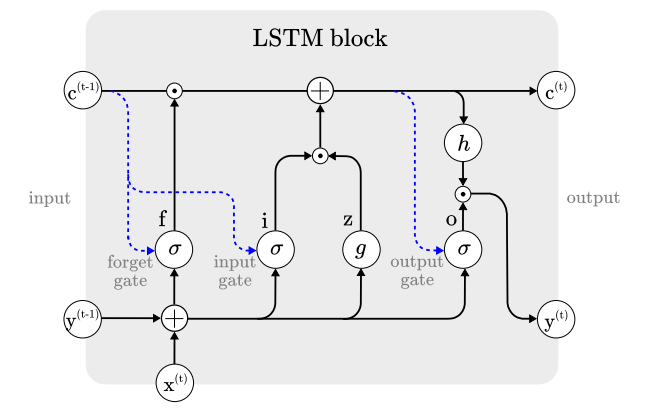
\includegraphics[scale=0.5]{gambar/bab2-lstm-model.png}
    \caption{How the LSTM architecture works}
    \label{fig:longshortterm}
\end{figure}

\emph{Long Short-Term Memory} (LSTM) is a special form of Recurrent Neural Network (RNN) that has feedback connection capabilities. This ability allows LSTM to remember information for long periods, thus solving problems with sequential or orderly characteristics. The advantage of LSTM compared to RNN is that LSTM has better and more effective memory abilities, minimizing information loss commonly occurring in processing long past information with RNN \cite{xia2020}. LSTM is very suitable for classifying sequential sign language. In Figure \ref{fig:longshortterm}, \emph{Long Short-Term Memory} is composed of several layers, including the block input, input gate, forget gate, cell, output gate, and block output, which can be sequentially formulated as follows:

\begin{equation}
    \label{eq:blockinputLSTM}
    x^{(t)} = g(W_z x^{(t)} + R_z y^{(t-1)} + b_z)
\end{equation}
\vspace{5mm}
\begin{equation}
    \label{eq:inputgateLSTM}
    i^{(t)} = \sigma(W_i x^{(t)} + R_i y^{(t-1)}+ p_i \odot c^{(t-1)} + b_i)
\end{equation}
\vspace{5mm}
\begin{equation}
    \label{eq:cellLSTM}
    c^{(t)} =  z^{(t)} \odot  i^{(t)} + z^{(t-1)} \odot  f^{(t)}
\end{equation}
\vspace{5mm}
\begin{equation}
    \label{eq:outputgateLSTM}
    o^{(t)} = \sigma(W_o x^{(t)} + R_o y^{(t-1)}+ p_o \odot c^{(t)} + b_o)
\end{equation}

\subsection{Intel \emph{Next Unit Computing} (NUC)}
\label{subsec:intelNUC}

Intel \emph{Next Unit Computing} (NUC) is a barebone computer designed by Intel. Intel NUC is a device that focuses on providing powerful computing in a practical size and can serve various user needs, from gaming to business to running complex applications. Intel NUC officially introduced this device in 2012 and marketed it publicly in early 2013 \cite{IntelNUC2020}. The first series of Intel NUC featured Sandy Bridge-based Celeron CPUs. Intel NUC has now evolved to the 12th generation, called Dragon Canyon, which features 12th generation Intel CPUs and PCI Express Gen 5 \cite{Halfacree2013}.
